	\section{ کدزنی و پیاده سازی‬}
	
	\subsection{بخش‌های ۱ تا ۴}
	
	\subsubsection{مقدمه}
	
	هدف این پروژه، پیاده‌سازی کامل یک شبکه عصبی از پایه و بدون استفاده از کتابخانه‌های آماده مانند TensorFlow یا PyTorch برای اهداف آموزشی است. این پروژه شامل مراحل مختلفی از جمله رگرسیون لجستیک، شبکه با لایه پنهان و در نهایت طبقه‌بندی چندکلاسه می‌باشد.
	
	\subsubsection{پیش‌پردازش داده‌ها}
	
	برای انجام این پروژه، از مجموعه داده \lr{CIFAR-10} استفاده شده است. تصاویر با استفاده از توابع موجود در \lr{torchvision} بارگذاری شده و به آرایه‌های \lr{CuPy} تبدیل گردیده‌اند تا از قدرت محاسباتی GPU بهره‌برداری شود.
	
	دیتاست به دو صورت مختلف برای وظایف دودویی و چندکلاسه پردازش شد:
	\begin{itemize}
		\item طبقه‌بندی دودویی: تصاویر هواپیما (\lr{airplane}) با برچسب صفر و سایر کلاس‌ها با برچسب یک.
		\item طبقه‌بندی چندکلاسه: برچسب‌ها به صورت \lr{one-hot} برای ده کلاس مختلف نگاشته شدند.
	\end{itemize}
	
	\subsubsection{بخش اول: رگرسیون لجستیک}
	
	در این مرحله، هدف تشخیص اینکه آیا یک تصویر متعلق به کلاس هواپیما است یا خیر می‌باشد. مدل تنها شامل یک لایه است با تابع فعال‌سازی سیگموئید:
		$$\sigma(z) = \frac{1}{1 + e^{-z}}$$
		\[\sigma^\prime = \sigma \times (1-\sigma)\]
	
	\[
	\hat{y} = \sigma(Wx + b)
	\]


	
	
	تابع خطای مورد استفاده، \lr{Binary Cross-Entropy} است:
	
	\[
	\mathcal{L}(y, \hat{y}) = - \frac{1}{N} \sum_{i=1}^N \left[ y_i \log(\hat{y}_i) + (1 - y_i) \log(1 - \hat{y}_i) \right]
	\]
	
	\subsubsection{آموزش مدل با گرادیان کاهشی}
	
	مدل \texttt{LogisticRegression} برای یادگیری رگرسیون لجستیک با استفاده از گرادیان کاهشی پیاده‌سازی شده است. مراحل کلیدی شامل موارد زیر است:
	
	\begin{itemize}
		\item \textbf{مقداردهی اولیه}: وزن‌ها با مقادیر کوچک تصادفی و بایاس با صفر مقداردهی می‌شوند.
		\item \textbf{پیش‌بینی}: محاسبه $z = XW + b$ و سپس $a = \sigma(z)$.
		\item \textbf{محاسبه گرادیان}:
		\[
		dz = \hat{y} - y,\quad dW = \frac{1}{m} X^T dz,\quad db = \frac{1}{m} \sum dz
		\]
		\item \textbf{به‌روزرسانی پارامترها}:
		\[
		W \leftarrow W - lr \cdot dW,\quad b \leftarrow b - lr \cdot db
		\]
		\item \textbf{آموزش}: اجرای مراحل فوق به‌صورت mini-batch در طول اپوک‌ها و ثبت دقت و زیان.
		\item \textbf{پیش‌بینی نهایی}: با آستانه ۰.۵، خروجی دودویی تولید می‌شود.
	\end{itemize}
	
	کلاس \texttt{SimpleLoader} برای تقسیم داده‌ها به دسته‌های تصادفی طراحی شده است.
	
	
	پارامترها با گرادیان نزولی به‌روزرسانی شدند.
	
	مدل با معیارهای مختلف بر روی داده آزمون ارزیابی شده است. برای تعیین بهترین آستانه طبقه‌بندی، جستجویی میان 0.1 تا 0.9 انجام شد. 
	
	\subsection*{نتایج ارزیابی پس از ۲۰۰ اپوک با \lr{lr=0.0001} و \lr{batch size=512}:}
	\begin{itemize}
		\item \textbf{بهترین آستانه}: \lr{0.50}
		\item \textbf{بهترین F1-score}: \lr{0.4460}
		\item \textbf{دقت آزمون}: \lr{0.8872}
	\end{itemize}
	
	\subsection*{ماتریس درهم‌ریختگی:}
	\begin{center}
		\begin{tabular}{|l|l|l|}
			\hline
			& Pred Other & Pred Airplane \\ \hline
			True Other    & 8418       & 582           \\ \hline
			True Airplane & 546        & 454           \\ \hline
		\end{tabular}
	\end{center}
	
	\subsection*{گزارش طبقه‌بندی:}
	\begin{center}
		\begin{tabular}{|l|l|l|l|l|}
			\hline
			& precision & recall & f1-score & support \\ \hline
			Other        & \lr{0.9391} & \lr{0.9353} & \lr{0.9372} & \lr{9000} \\ \hline
			Airplane     & \lr{0.4382} & \lr{0.4540} & \lr{0.4460} & \lr{1000} \\ \hline
			\textbf{accuracy} & & & \textbf{\lr{0.8872}} & \lr{10000} \\ \hline
			macro avg    & \lr{0.6887} & \lr{0.6947} & \lr{0.6916} & \lr{10000} \\ \hline
			weighted avg & \lr{0.8890} & \lr{0.8872} & \lr{0.8881} & \lr{10000} \\ \hline
		\end{tabular}
	\end{center}
	
\begin{figure}[h]
	\centering
	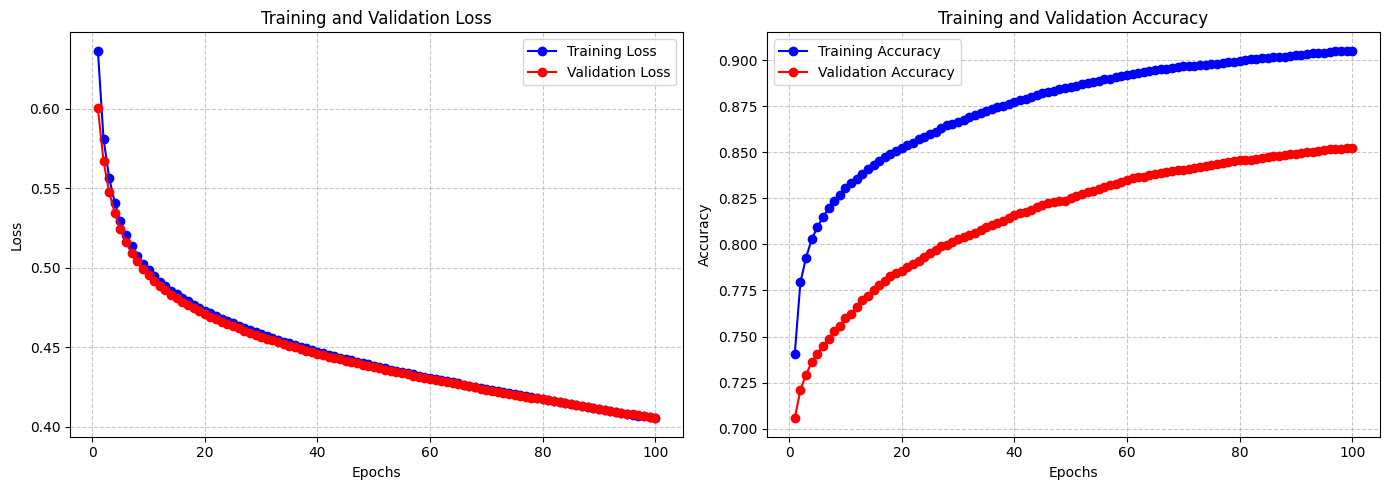
\includegraphics[width=0.7\linewidth]{images/task1-2}
	\caption{تغییرات دقت و هزینه در طی آموزش با مدل رگرسیون لجستیک}
	\label{fig:task1-1}
\end{figure}


	\subsubsection{بخش دوم: شبکه با یک لایه پنهان}
	
	در این بخش، مدل با افزودن یک لایه پنهان با 64 نورون توسعه یافت. معماری شبکه به صورت زیر است:
	
	\[
	\begin{aligned}
		Z_1 &= W_1 X + b_1 \\
		A_1 &= \sigma(Z_1) \\
		Z_2 &= W_2 A_1 + b_2 \\
		A_2 &= \sigma(Z_2)
	\end{aligned}
	\]
	
	در اینجا نیز از سیگموئید به عنوان تابع فعال‌سازی استفاده شده و آموزش با الگوریتم گرادیان نزولی انجام شده است.
	
\begin{figure}[h]
	\centering
	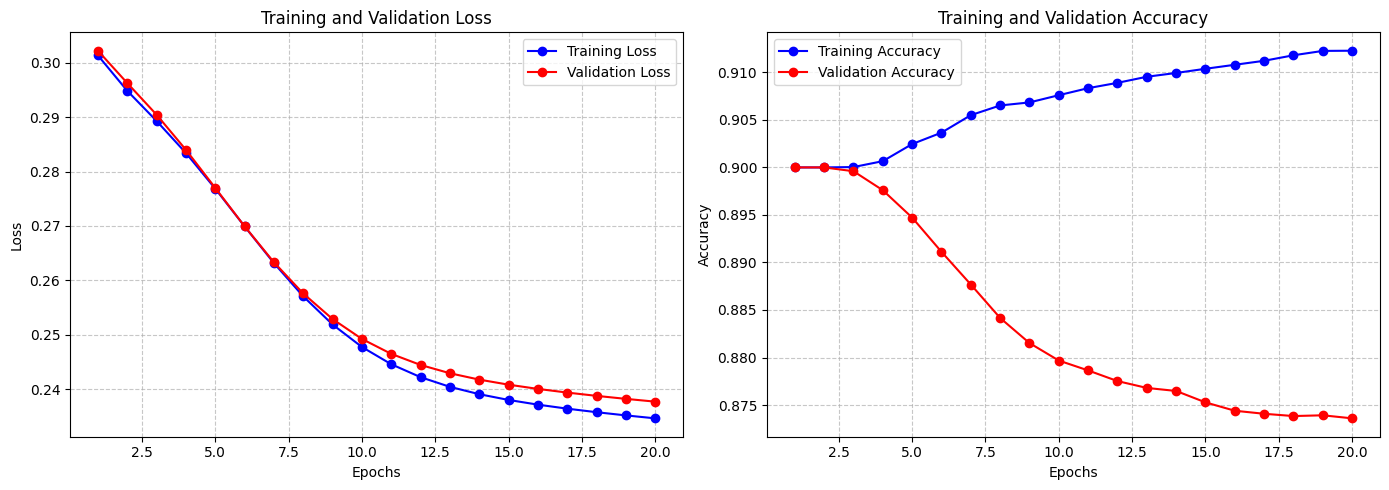
\includegraphics[width=0.7\linewidth]{images/task2-1}
	\caption{تغییرات دقت و هزینه در طی آموزش با مدل رگرسیون لجستیک چند لایه}
	\label{fig:task2-1}
\end{figure}


\begin{lstlisting}
	Classification Report:
	              precision    recall  f1-score   support
	
	Airplane         0.7000    0.2310    0.3474      1000
	Not Airplane     0.9205    0.9890    0.9535      9000
	
	accuracy                             0.9132     10000
	macro avg        0.8102    0.6100    0.6504     10000
	weighted avg     0.8984    0.9132    0.8929     10000
	
\end{lstlisting}

\begin{figure}[h]
	\centering
	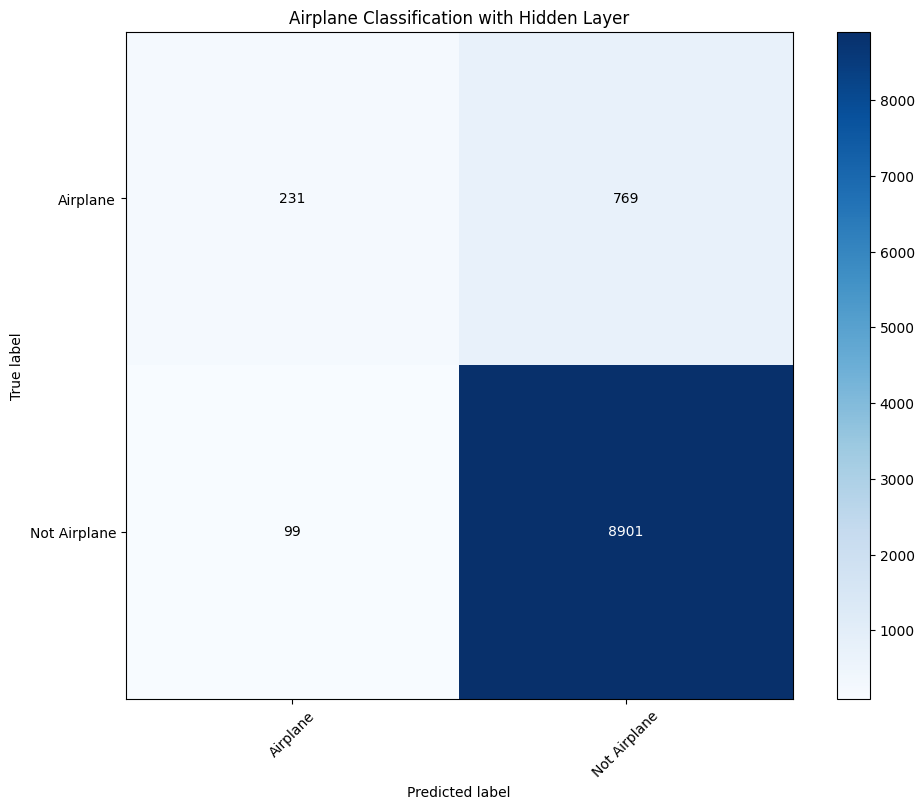
\includegraphics[width=0.5\linewidth]{images/task2-3}
	\caption{ماتریس آشفتگی برای مدل رگرسیون لاجستیک چند لایه بعد ۲۰ ایپاک}
	\label{fig:task2-3}
\end{figure}




	\subsubsection{بخش سوم: طبقه‌بندی چندکلاسه}
	
	در این مرحله، شبکه برای شناسایی تمامی ۱۰ کلاس \lr{CIFAR-10} طراحی شد. خروجی شبکه دارای ۱۰ نورون با تابع فعال‌سازی \lr{Softmax} است:
	
	\[
	\text{Softmax}(z_i) = \frac{e^{z_i}}{\sum_{j=1}^{10} e^{z_j}}
	\]
	
	تابع هزینه مورد استفاده، \lr{Categorical Cross-Entropy} است.
	
		
	\begin{figure}[h]
		\centering
		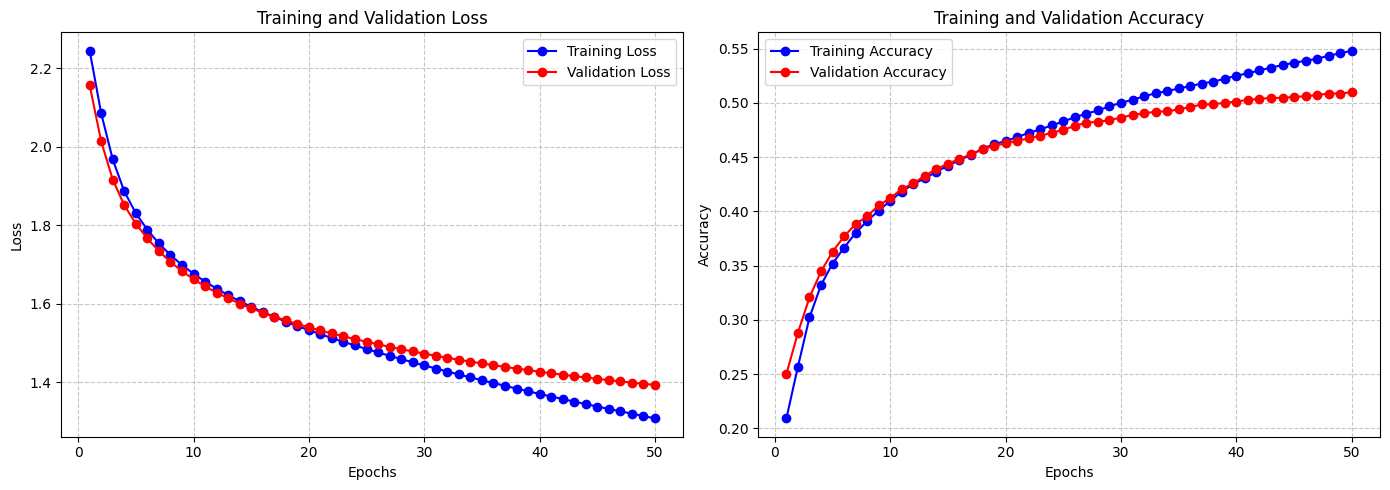
\includegraphics[width=0.7\linewidth]{images/task3-1}
		\caption{تغییرات دقت و هزینه در طی آموزش با مدل رگرسیون وان‌هات چند لایه}
		\label{fig:task3-1}
	\end{figure}
	
	
	
	\begin{lstlisting}
		Classification Report:
		precision                  recall  f1-score   support
		
		airplane         0.5959    0.5840    0.5899      1000
		automobile       0.6030    0.5970    0.6000      1000
		bird             0.4269    0.3270    0.3703      1000
		cat              0.3580    0.3430    0.3504      1000
		deer             0.4403    0.3800    0.4079      1000
		dog              0.4317    0.3920    0.4109      1000
		frog             0.4860    0.6400    0.5524      1000
		horse            0.5580    0.5720    0.5649      1000
		ship             0.5958    0.6750    0.6329      1000
		truck            0.5547    0.5880    0.5709      1000
		
		accuracy                             0.5098     10000
		macro avg        0.5050    0.5098    0.5051     10000
		weighted avg     0.5050    0.5098    0.5051     10000
		
	\end{lstlisting}
	
	\begin{figure}[h]
		\centering
		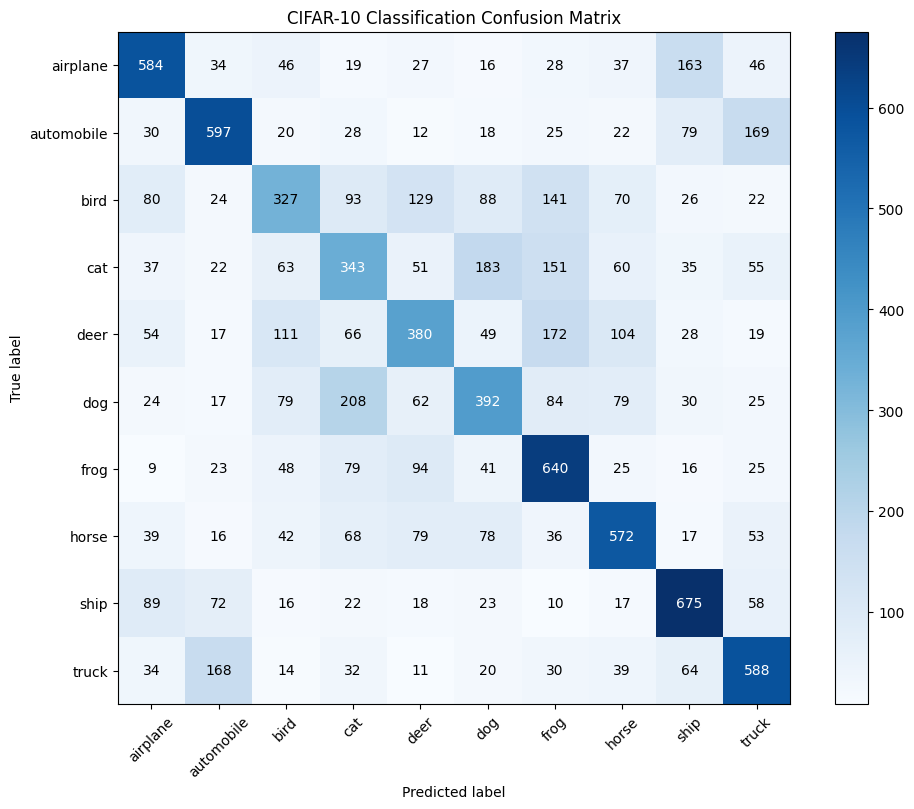
\includegraphics[width=0.8\linewidth]{images/task3-2}
		\caption{ماتریس آشفتگی برای مدل رگرسیون وان هات چند لایه بعد ۵۰ ایپاک}
		\label{fig:task3-2}
	\end{figure}
	
	
	
	
	
\subsubsection{بخش چهارم: مقایسه‌ی ویژگی‌های شبکه عصبی نیمه پیشرفته}
	
	در این بخش، یک شبکه عصبی نیمه پیشرفته با قابلیت استفاده از بهینه‌سازهای مختلف و توابع فعال‌سازی گوناگون پیاده‌سازی شده است. ساختار شبکه به‌گونه‌ای طراحی شده که از وزن‌دهی اولیه مناسب، ذخیره‌سازی گرادیان‌ها، و بهینه‌سازهای مدرن مانند Adam پشتیبانی می‌کند. 
	
	\subsubsection{توابع فعال‌سازی}
	
	توابع فعال‌سازی نقش مهمی در آموزش شبکه‌های عصبی ایفا می‌کنند. در این پروژه از سه تابع فعال‌سازی پرکاربرد شامل \lr{ReLU}، \lr{Sigmoid}، و \lr{Tanh} استفاده شده است.
	
	\begin{itemize}
		\item \textbf{تابع \lr{Sigmoid}:}
		\[
		\sigma(x) = \frac{1}{1 + e^{-x}}, \quad \sigma'(x) = \sigma(x)(1 - \sigma(x))
		\]
		
		\item \textbf{تابع \lr{Tanh}:}
		\[
		\tanh(x) = \frac{e^x - e^{-x}}{e^x + e^{-x}}, \quad \frac{d}{dx} \tanh(x) = 1 - \tanh^2(x)
		\]
		
		\item \textbf{تابع \lr{ReLU}:}
		\[
		f(x) = \max(0, x), \quad f'(x) = \begin{cases}
			1 & x > 0 \\
			0 & x \leq 0
		\end{cases}
		\]
	\end{itemize}

	
	در تحلیل تجربی، تابع ReLU به‌دلیل سادگی محاسباتی و اجتناب از مشکل ناپدید شدن گرادیان‌ها عملکرد برتری نسبت به سایر توابع نشان داد.
	
	\subsubsection{الگوریتم‌های بهینه‌سازی}
	
	در این پروژه سه الگوریتم زیر پیاده‌سازی و بررسی شده‌اند:
	\begin{enumerate}
		\item \lr{SGD}:
		به‌روزرسانی وزن‌ها به‌صورت مستقیم و بر پایه گرادیان فعلی صورت می‌گیرد:
		\[
		\theta = \theta - \eta \nabla_\theta J(\theta)
		\]
		که در آن \(\eta\) نرخ یادگیری و \(J(\theta)\) تابع هزینه است.
		
		\item \lr{Momentum}:
		این روش برای بهبود همگرایی، از سرعت قبلی استفاده می‌کند:
		\[
		v_t = \gamma v_{t-1} - \eta \nabla_\theta J(\theta) \quad,\quad \theta = \theta + v_t
		\]
		که در آن \(\gamma\) ضریب مومنتوم است.
		\item. \lr{Adam}:
		این روش تخمین‌هایی از میانگین و واریانس لحظه‌ای گرادیان‌ها ذخیره می‌کند:
		\[
		m_t = \beta_1 m_{t-1} + (1 - \beta_1) g_t
		\]
		\[
		v_t = \beta_2 v_{t-1} + (1 - \beta_2) g_t^2
		\]
		\[
		\hat{m}_t = \frac{m_t}{1 - \beta_1^t}, \quad \hat{v}_t = \frac{v_t}{1 - \beta_2^t}
		\]
		\[
		\theta = \theta - \eta \frac{\hat{m}_t}{\sqrt{\hat{v}_t} + \epsilon}
		\]
		\begin{figure}[h]
			\centering
			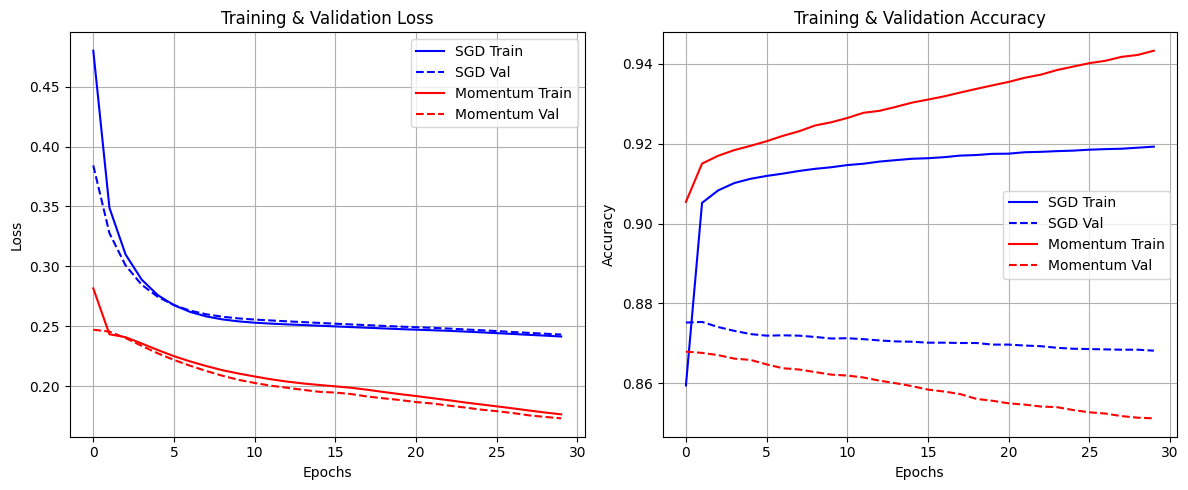
\includegraphics[width=0.7\linewidth]{images/task4-3}
			\caption{مقایسه‌ی همگرایی SGD و تکانه با فعال‌سازهای یکسان در دو لایه در داده‌های تست و آموزش}
			\label{fig:task4-3}
		\end{figure}
		
	
	\end{enumerate}
	

	
	
	
	\subsubsection{مقداردهی اولیه وزن‌ها}
	
	برای بهبود عملکرد یادگیری، از دو روش مقداردهی اولیه استفاده شده است:
	
	\begin{itemize}
		\item \textbf{He Initialization} برای توابع ReLU:
		\[
		\text{Var}(w) = \frac{2}{n_{\text{in}}}
		\]
		
		\item \textbf{Xavier Initialization} برای توابع Sigmoid و Tanh:
		\[
		\text{Var}(w) = \frac{1}{n_{\text{in}}}
		\]
	\end{itemize}
	
	\begin{figure}[h]
		\centering
		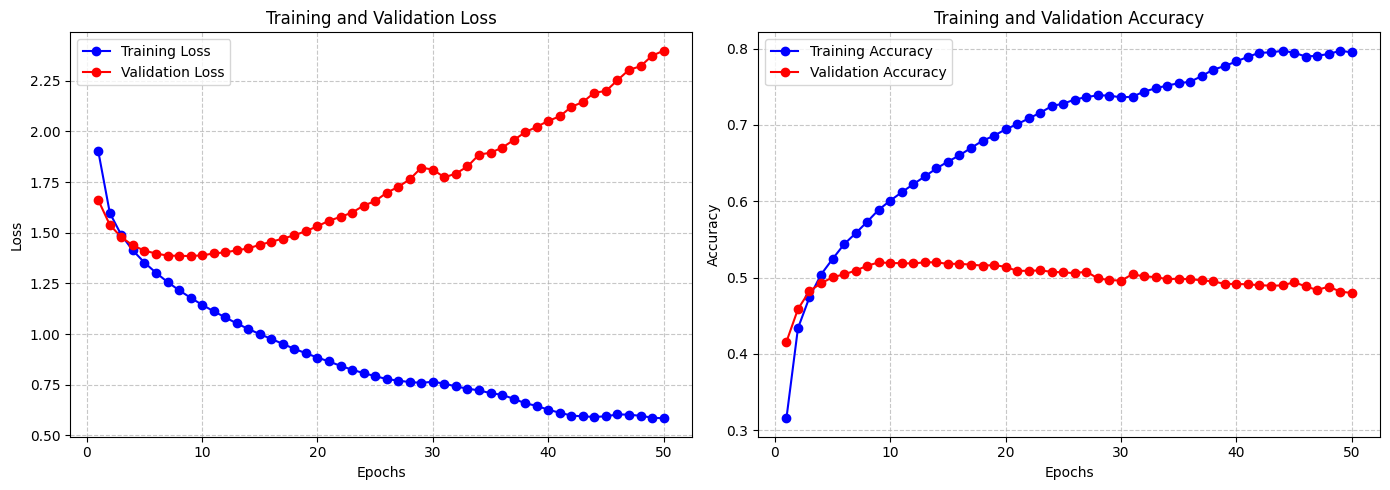
\includegraphics[width=0.7\linewidth]{images/task4-4}
		\caption{اثر مقداردهی اولیه He در یک شبکه دو لایه با بهینه‌ساز تکانه در ۳۰ ایپاک}
		\label{fig:task4-4}
	\end{figure}
	
	
	\subsubsection{مقایسه تجربی توابع فعال‌سازی}
	
	در بخش سوم، برای مقایسه عملکرد توابع فعال‌سازی، سه شبکه با ساختار یکسان ولی با توابع ReLU، Sigmoid، و Tanh آموزش داده شد. نتایج نشان دادند که:
	
	\begin{itemize}
		\item ReLU منجر به همگرایی سریع‌تر و دقت بالاتر در داده‌های تست شد.
		\item Sigmoid به‌دلیل ناپدید شدن گرادیان در لایه‌های عمیق ضعیف‌ترین عملکرد را داشت.
		\item Tanh عملکردی بین دو تابع دیگر ارائه داد.
	\end{itemize}
		\begin{figure}[h]
		\centering
		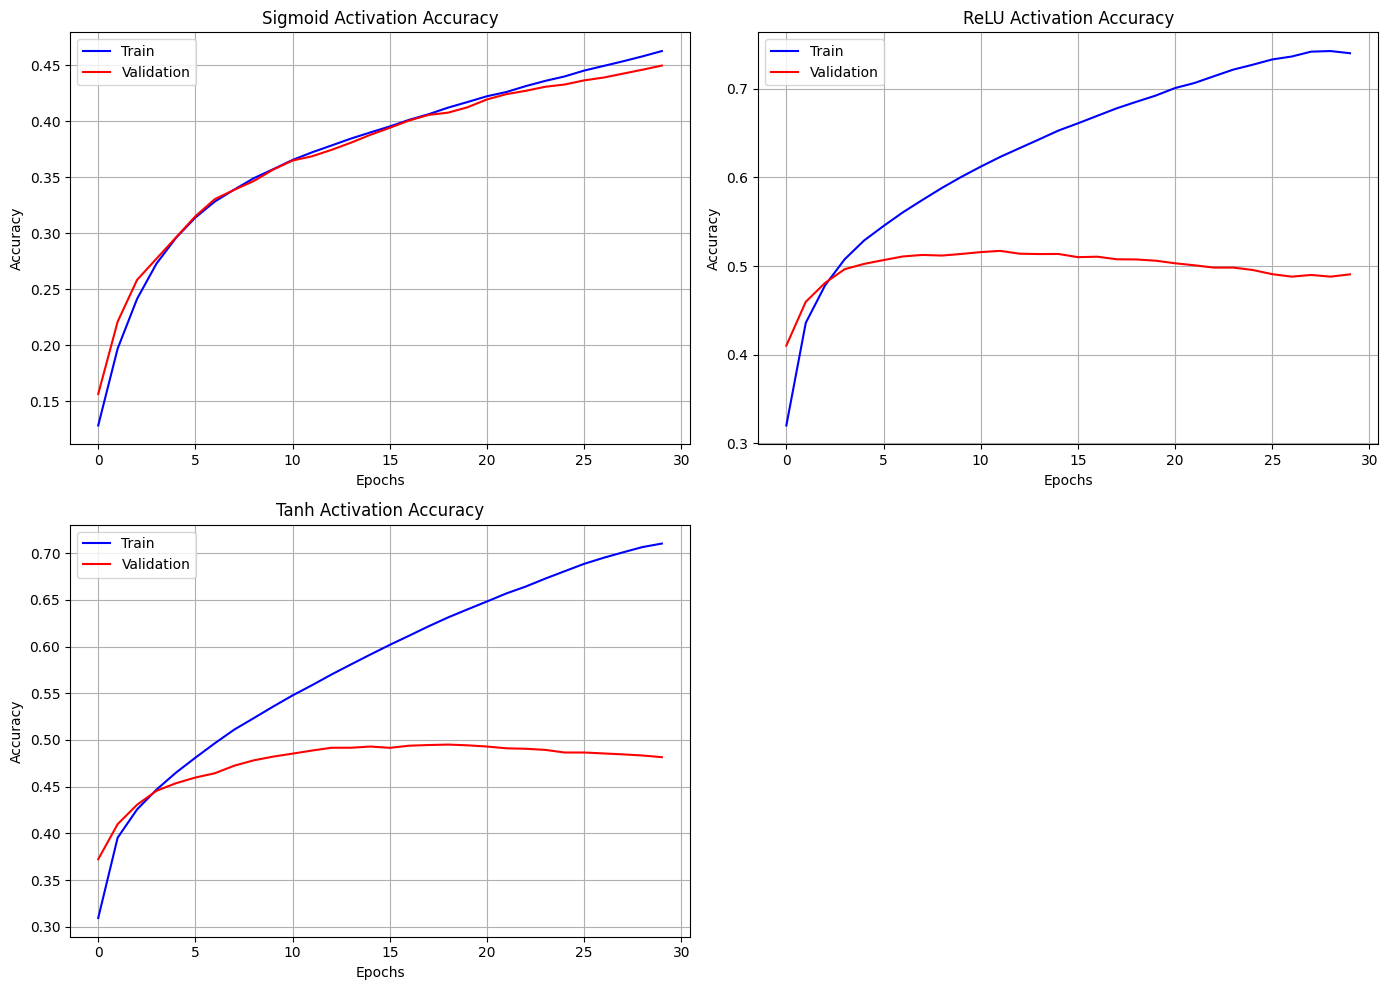
\includegraphics[width=0.7\linewidth]{images/task4-2}
		\caption{مقایسه‌ی همگرایی توابع فعالسازی متفاوت با ۳۰ ایپاک}
		\label{fig:task4-2}
	\end{figure}
	
	نتایج در قالب نمودارهای دقت در طول اپوک‌ها رسم گردیدند.
	
	\subsubsection{مقایسه تجربی بهینه‌سازها}
	
	در بخش پایانی، عملکرد سه الگوریتم \lr{SGD}، \lr{Momentum} و \lr{Adam} بر روی یک شبکه سه‌لایه آزمایش شد. نتایج حاکی از آن بود که:
	
	\begin{itemize}
		\item Adam در اکثر موارد سریع‌تر همگرا شد و به دقت بالاتری رسید.
		\item Momentum پایداری بهتری نسبت به SGD داشت.
		\item استفاده از بهینه‌ساز مناسب نقش مهمی در کیفیت آموزش دارد.
	\end{itemize}
		
	\begin{figure}[h]
		\centering
		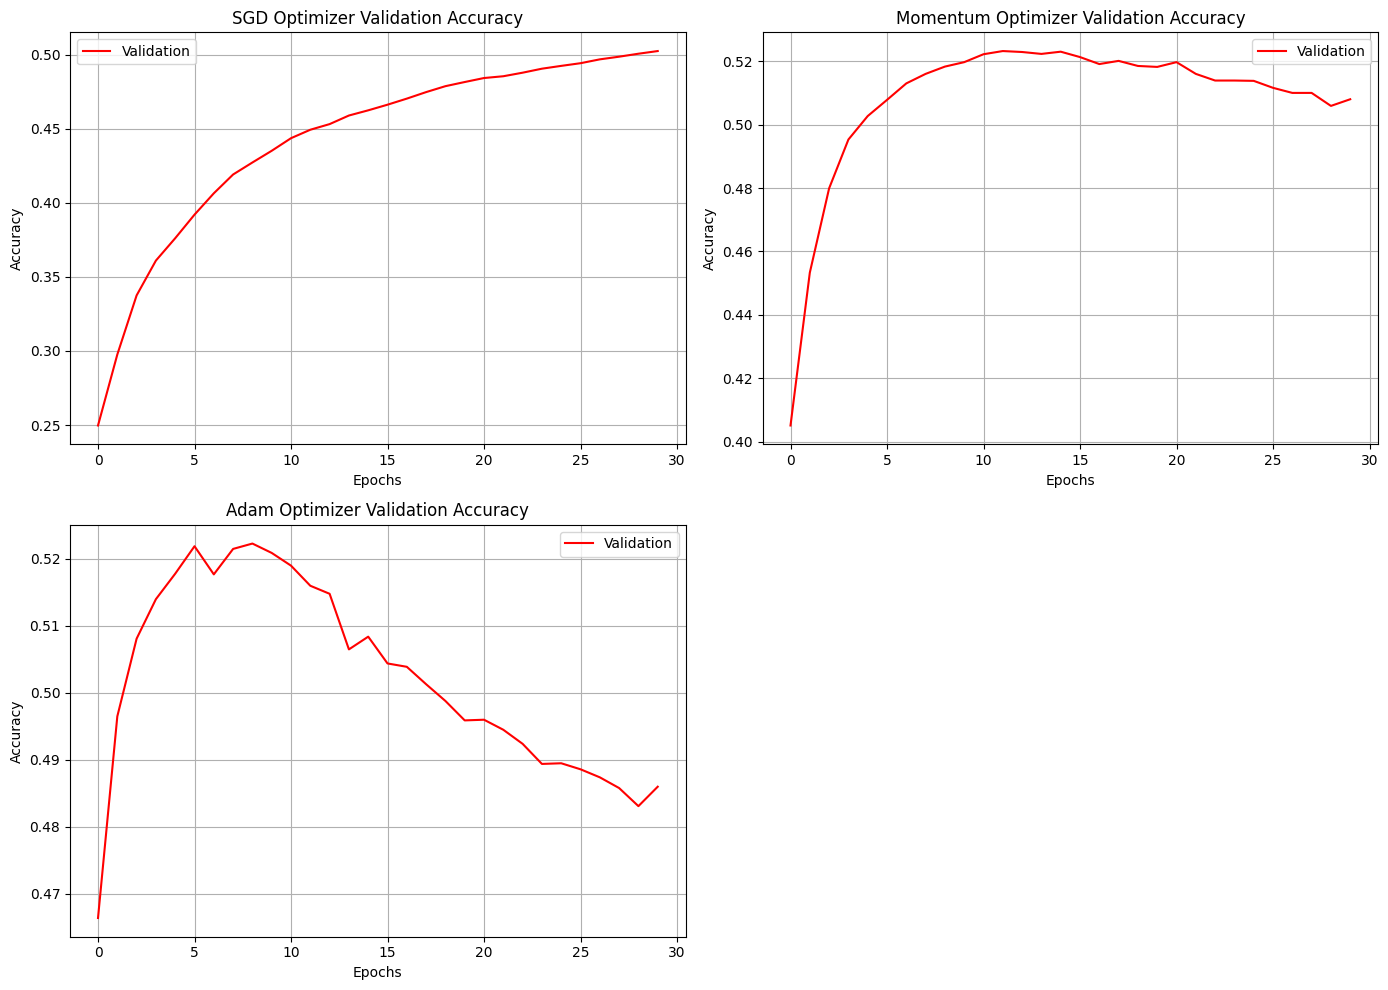
\includegraphics[width=0.7\linewidth]{images/task4-1}
		\caption{مقایسه‌ی همگرایی بین بهینه‌سازهای مختلف در ۳۰ ایپاک}
		\label{fig:task4-1}
	\end{figure}
	
	
	مدل طراحی‌شده در این پروژه به‌دلیل ساختار ماژولار و قابل گسترش، قابلیت استفاده در کاربردهای مختلف را دارد. نتایج تجربی نشان دادند که انتخاب دقیق تابع فعال‌سازی، مقداردهی اولیه مناسب، و الگوریتم بهینه‌سازی مؤثر نقش کلیدی در موفقیت مدل ایفا می‌کند.
	


\subsection{بخش ۵: آموزش مدل از طریق شبکه عصبی CNN}



		\subsubsection{تنظیم داده‌ها و بارگذاری CIFAR-10}

		مجموعه‌داده CIFAR-10 را با نرمال‌سازی مناسب بارگذاری کنید و DataLoader‌‌های آموزش و تست را با اندازه بچ و شافل دلخواه ایجاد نمایید.

		\lstinputlisting[language=Python, caption=تعریف \lr{transforms} و \lr{DataLoader}]{./scripts/data\_loader\_cifar10.py}


		% Task 2
		\subsubsection{تعریف معماری ساده CNN}

		یک کلاس PyTorch از نوع \lr{nn.Module} با ساختار زیر پیاده‌سازی کنید:
		\begin{itemize}
			\item \lr{Conv2d} با 32 فیلتر، کرنل $3\times3$, فعال‌سازی \lr{ReLU}
			\item \lr{MaxPool2d} با کرنل $2\times2$
			\item \lr{Conv2d} با 64 فیلتر، کرنل $3\times3$, فعال‌سازی \lr{ReLU}
			\item \lr{MaxPool2d} با کرنل $2\times2$
			\item \lr{Flatten()} و دو لایه تمام‌متصل 128 و 10 نورونی (Softmax خروجی)
		\end{itemize}

		\lstinputlisting[language=Python, caption=کلاس \lr{SimpleCNN}]{./scripts/simple_cnn.py}


		% Task 3
		\subsubsection{حلقه آموزش مدل}

		حلقه آموزشی را با تابع هزینه \lr{CrossEntropyLoss} و بهینه‌ساز \lr{SGD} با \lr{Momentum} پیاده کنید. در هر صد گام آموزشی، میانگین \lr{loss} را چاپ نمایید.

		\lstinputlisting[language=Python, caption=حلقه آموزش \lr{train loop}]{./scripts/train_cnn.py}


		% Task 4
		\subsubsection{ارزیابی مدل و گزارش دقت}

		مدل آموزش‌دیده را روی مجموعه تست ارزیابی کنید و دقت نهایی را محاسبه و چاپ کنید. سپس وزن‌های مدل را ذخیره نمایید.

		\lstinputlisting[language=Python, caption=ارزیابی و ذخیره مدل]{./scripts/evaluate_cnn.py}


		% Task 5
		\subsubsection{گزارش معماری و تحلیل نتایج}

		یک گزارش مختصر بنویسید که شامل معماری نهایی، جزییات پیاده‌سازی، روند آموزش و نتایج ارزیابی باشد. همچنین مزایا و معایب استفاده از CNN را در مقایسه با پرسپترون چندلایه مورد بحث قرار دهید.

		\subsubsection{مزایا و معایب استفاده از \lr{CNN} در مقابل یک پرسپترون چندلایه}

		\vspace{0.5em}
		\noindent
		\textbf{مزایا:}
		\begin{itemize}
			\item \textbf{استخراج ویژگی‌های مکانی:} لایه‌های کانولوشنال با حفظ ساختار دوبعدی تصویر، الگوهای محلی مانند لبه‌ها و بافت‌ها را بهتر استخراج می‌کنند، در حالی که MLP تصویر را صاف‌شده دریافت می‌کند.
			\item \textbf{کاهش پارامترها:} با اشتراک وزن در فیلترها، تعداد پارامترها به‌طور قابل‌توجهی کمتر از MLP بوده و خطر بیش‌برازش کاهش می‌یابد.
			\item \textbf{مقیاس‌پذیری:} استفاده از pooling و فیلترهای محلی باعث می‌شود CNN بتواند روی تصاویر بزرگ‌تر یا پیچیده‌تر نیز کارایی مناسبی داشته باشد.
			\item \textbf{تعمیم بهتر:} CNN در برابر تغییرات کوچک در تصویر (جابجایی، چرخش، تغییر نور) مقاوم‌تر است و به همین دلیل در داده‌های بصری عملکرد بهتری دارد.
		\end{itemize}

		\noindent
		\textbf{معایب:}
		\begin{itemize}
			\item \textbf{پیچیدگی پیاده‌سازی:} طراحی معماری CNN اعم از انتخاب تعداد لایه‌ها، فیلترها و سایر ابرپارامترها نیازمند تجربه و آزمون‌وخطای بیشتری است.
			\item \textbf{زمان آموزش:} محاسبات کانولوشن هزینه‌برتر از ضرب‌های برداری ساده در MLP بوده و ممکن است زمان آموزش طولانی‌تری داشته باشد.
			\item \textbf{وابستگی به GPU:} برای آموزش سریع و مؤثر CNN معمولاً نیاز به شتاب‌دهنده‌هایی مانند GPU است، در حالی که MLP را می‌توان حتی روی CPU اجرا کرد.
		\end{itemize}
